%---------------------------------------------------------------------------------------------------
% Voreinstellungen (Layout, neue Befehle, etc.)
%---------------------------------------------------------------------------------------------------

%---------------------------------------------------------------------------------------------------
% Einstellungen
% (gelten nur in Zusammenarbeit mit pdflatex)
%---------------------------------------------------------------------------------------------------
\documentclass[
  pagesize,	                                           % flexible Auswahl des Papierformats
  a4paper,  	                                         % DIN A4
  oneside,    	                                       % einseitiger Druck
  BCOR5mm,      	                                     % Bindungskorrektur
  headsepline,                                         % Strich unter der Kopfzeile
  12pt,                                                % 12pt Schriftgr��e
	halfparskip,                                         % Europ�ischer Satz: Abstand zwischen Abs�tzen
	abstracton,																					 % Spezielle Formatierung, die erlaubt, dass die
																											 % Zusammenfassung vor dem Inhaltsverzeichnis steht
	%draft,																							 % Es handelt sich um eine Vorabversion	
	final,																							 % Es handelt sich um die endg�ltige Version
	liststotoc,																					 % Tabellen- und Abbildungsverzeichnis im 																																 % Inhaltsverzeichnis
	idxtotoc,																						 % Index im Inhaltsverzeichnis	
  bibtotoc,                                            % Literaturverzeichnis im Inhaltsverzeichnis  
]{scrreprt}                                            % KOMA-Scriptklasse Report

%---------------------------------------------------------------------------------------------------
\usepackage[english,ngerman]{babel}                    % deutsche Trennmuster
\usepackage[T1]{fontenc}                               % EC-Schriften, Trennstellen nach Umlauten
\usepackage[latin1]{inputenc}                          % direkte Umlauteingabe (� statt "a)
                                                       % latin1/latin9 f�r unixoide Systeme
                                                       % (latin1 ist auch unter Win verwendbar)
                                                       % ansinew f�r Windows
                                                       % applemac Macs
                                                       % cp850 OS/2
\usepackage{times}              											 % Schriften Paket
\usepackage{array,ragged2e} 													 % Wichtig f�r Abstandsformatierung
\usepackage{float}
\usepackage{comment}
%---------------------------------------------------------------------------------------------------
\usepackage{cmbright}                                  % serifenlose Schrift als Standard
                                                       % + alle f�r TeX ben�tigten mathematischen
                                                       %   Schriften einschlie�lich der AMS-Symbole
\usepackage[scaled=.90]{helvet}                        % skalierte Helvetica als \sfdefault
\usepackage{courier}                                   % Courier als \ttdefault

%---------------------------------------------------------------------------------------------------
\usepackage[automark]{scrpage2}                        % Anpassung der Kopf- und Fu�zeilen
\usepackage{xspace}                                    % Korrekter Leerraum nach Befehlsdefinitionen
\usepackage{setspace}																	 % Dieses Package brauchen wir f�r den 				
\usepackage[pdftex]{graphicx}
\usepackage[absolute,overlay]{textpos}         
\usepackage[final]{pdfpages}																											 % anderthalbzeiligen Abstand.
\usepackage{natbib}                                    % Neuimplementierung des \cite-Kommandos
\usepackage{bibgerm}       											       % Deutsche Bezeichnungen
\usepackage[absolute]{textpos}                         % placing boxes at absolute positions
\usepackage[final]{pdfpages}                           % include pages of external PDF documents
\usepackage{tabularx}                                  % Spaltenbreite bis zur Seitenbreite dehnen
\usepackage{makeidx}													% Paket zur Erstellung eines Stichwortverzeichnisses

% Listing START
\usepackage{listings}
\usepackage{xcolor}	
												% Paket zur Erstellung eines Stichwortverzeichnisses
\colorlet{punct}{red!60!black}
\definecolor{background}{HTML}{EEEEEE}
\definecolor{delim}{RGB}{20,105,176}

\lstdefinelanguage{json}{
    basicstyle=\normalfont\ttfamily,
    numbers=left,
    numberstyle=\scriptsize,
    stepnumber=1,
    numbersep=8pt,
    showstringspaces=false,
    breaklines=true,
    frame=lines,
    backgroundcolor=\color{background},
    literate=
      {:}{{{\color{punct}{:}}}}{1}
      {,}{{{\color{punct}{,}}}}{1}
      {\{}{{{\color{delim}{\{}}}}{1}
      {\}}{{{\color{delim}{\}}}}}{1}
      {[}{{{\color{delim}{[}}}}{1}
      {]}{{{\color{delim}{]}}}}{1},
}
% Listing END
\makeindex																						 % Automatische Erstellung des Stichwortverzeichnis
\usepackage[intoc,
						english,
						prefix]{nomencl}
\makenomenclature

%---------------------------------------------------------------------------------------------------
 \usepackage{graphicx}                                 % Zur Einbindung von PDF-Bildern
 \usepackage[colorlinks,															 % Einstellen und Laden des Hyperref-Pakets
	pdftex,
	bookmarks,
	bookmarksopen=false,
	bookmarksnumbered,
	citecolor=blue,
	linkcolor=blue,
	urlcolor=blue,
	filecolor=blue,
	linktocpage,
  pdfstartview=Fit,                                  % startet mit Ganzseitenanzeige    
	pdfsubject={Multiagentensystemgest�tzte Clusteranalyse},
	pdftitle={Diplomarbeit im Fachbereich Elektrotechnik \& Informatik an der HAW-Hamburg},
	pdfauthor={Bj�rn Jensen, http://www.mirou.de}]{hyperref}
 \pdfcompresslevel=9
 
%---------------------------------------------------------------------------------------------------
% Inhaltsverzeichnis und Abschnittnummerierung
%---------------------------------------------------------------------------------------------------
\setcounter{secnumdepth}{2}   % Ich habe recht kurze Kapitel. Die sollen nicht durchnummeriert sein.
\setcounter{tocdepth}{2}

%---------------------------------------------------------------------------------------------------
% Abbildungsverzeichnis
%---------------------------------------------------------------------------------------------------
\graphicspath{{graphics/}}

%---------------------------------------------------------------------------------------------------
% Kopf- und Fu�zeilen
%---------------------------------------------------------------------------------------------------
\pagestyle{scrheadings}
\clearscrheadings
\clearscrplain
\clearscrheadfoot
\ohead{\pagemark}
\ihead{\headmark}

%---------------------------------------------------------------------------------------------------
% Neue Befehle
%---------------------------------------------------------------------------------------------------
%---------------------------------------------------------------------------------------------------
% Neue Befehle
%---------------------------------------------------------------------------------------------------

%---------------------------------------------------------------------------------------------------
% Umbenennen des Symbolverzeichnisses
%---------------------------------------------------------------------------------------------------
\renewcommand{\nomname}{Glossar}				% Das Symbolverzeichnis heisst nun "Glossar"
\renewcommand{\nomlabel}[1]{						% Die zu erkl�renden Begriffe sind nun fett hervorgehoben
	\hfil \textbf{#1} \hfil
}

%---------------------------------------------------------------------------------------------------
% Ein paar ganz n�tzliche Befehle von Lars M�hlmann
%---------------------------------------------------------------------------------------------------
%f�r Kommentare 
\newcommand{\colb}{\color{green}}
\newcommand{\colbl}{\color{black}}

%---------------------------------------------------------------------------------------------------
% Befehle zum Erstellen des Index
% \addIndexEntry{Eintrag in den Index}
% \addSubIndexEntry{Eintrag in den Index}{Eintrag des �bergeordneten Eintrags}
%---------------------------------------------------------------------------------------------------
\newcommand{\addIndexEntry}[1]{#1\index{#1}}
\newcommand{\addSubIndexEntry}[2]{#1\index{#2!#1}}

%---------------------------------------------------------------------------------------------------
% LaTeX in eigenem Font
%---------------------------------------------------------------------------------------------------
\newcommand{\myLatex}{
	{\rmfamily\LaTeX\xspace}
}

%---------------------------------------------------------------------------------------------------
% Befehl zum Erstellen und Hervorheben eines Zitats
% Parameter:
% 1. Zitat
% 2. Author
% 3. Quelle
%---------------------------------------------------------------------------------------------------
\newcommand{\myCitation}[3]{
	\begin{flushright}
	\begin{minipage}{.4\linewidth}
		\footnotesize\rmfamily\itshape 
		#1 \\
		\RaggedLeft #2 \\
		#3
	\end{minipage}
	\end{flushright}
	\nobreakspace
}

%---------------------------------------------------------------------------------------------------
% Erstellung von Deckblatt (Seite 1) und Titelblatt (Seite 2)
%---------------------------------------------------------------------------------------------------
\newcommand{\createCoverAndTitlePage}[7]{
	\createCover{#1}{#2}{#3}{#4}
	\createTitlePage{#1}{#2}{#3}{#4}{#5}{#6}{#7}
}

%---------------------------------------------------------------------------------------------------
% Erstellung von Deckblatt (Seite 1) 
% Anwendung:
% \createCover{Art der Arbeit}{Typ der Arbeit}{Autor}{Titel}
%---------------------------------------------------------------------------------------------------
\newcommand{\createCover}[4]{
	\thispagestyle{empty}
	\begin{titlepage}

	\setlength{\TPHorizModule}{1mm}
	\setlength{\TPVertModule}{1mm}
	\textblockorigin{0mm}{0mm} % start everything near the top-left corner

	% Art der Arbeit
	\begin{textblock}{111}(83,115)
		\begin{minipage}[c][1,78cm][c]{11,09cm}		
  		\fontsize{22pt}{20pt}
  		\selectfont
  		\begin{center}
  		#1#2
  		\end{center}
		\end{minipage}
	\end{textblock}

	% Name & Titel
	\begin{textblock}{111}(83,131)
		\begin{minipage}[c][4,81cm][t]{11,09cm}	
		\linespread{1.2}	
    		\fontsize{16pt}{14pt}    
    		\selectfont
    		\begin{center}
    			#3 \\ \medskip    
    			#4
    		\end{center}
    		\end{minipage}
	\end{textblock}
	\begin{textblock}{111}(35,260)
		\begin{minipage}[c][1,5cm][t]{7,0cm}		
  		\fontsize{10pt}{10pt}
  		\selectfont
		\textit{
  		Fakult\"at Technik und Informatik \\
  		Department Informations- und \\
		Elektrotechnik}
		\end{minipage}
	\end{textblock}


	\begin{textblock}{111}(125,260)
		\begin{minipage}[c][1,5cm][t]{7,0cm}		
  		\fontsize{10pt}{10pt}
  		\selectfont
		\textit{
  		Faculty of Engineering and Computer Science\\
  		Department of Information and \\
		Electrical Engineering}
		\end{minipage}
	\end{textblock}

	\end{titlepage}
%---------------------------------------------------------------------------------------------------
% Wichtig! Entsprechendes Auskommentieren!
%---------------------------------------------------------------------------------------------------
 
\includepdf{pdf/DeckblattFarbe} 		% zum Ausdruck auf blanko Papier
  % **************************************************************************************
  % Originaldeckblatt mit WORD Vorlage drucken, da nur dort offizieller Schrifttyp vorhanden
  % **************************************************************************************
}

%---------------------------------------------------------------------------------------------------
% Erstellung von Titelblatt (Seite 2) 
% Anwendung:
% \createTitlePage{Art der Arbeit}{Typ der Arbeit}{Author}{Titel}{Studiengang}{Erstpr�fer}{Zweitpr�fer}
%---------------------------------------------------------------------------------------------------
\newcommand{\createTitlePage}[8]{
	\thispagestyle{empty}

	\setlength{\TPHorizModule}{1mm}
	\setlength{\TPVertModule}{\TPHorizModule}
	\textblockorigin{0mm}{0mm} % start everything near the top-left corner

	% Name & Titel
	\begin{textblock}{130}(40,63)
		\begin{minipage}[c][5,9cm][t]{13cm}
			\begin{center}
			\linespread{1.2}
			\fontsize{18pt}{18pt}
  		\selectfont
  		#3 \\ \medskip
  		\fontsize{16pt}{16pt}
  		#4
  		\end{center}
		\end{minipage}  	
	\end{textblock}

	% Infos zur Arbeit und zum Deapratment
	\begin{textblock}{126}(32,214)
  	\begin{minipage}[t][6,72cm][l]{12,57cm}
    	\fontsize{12pt}{12pt}
    	\selectfont
    	#1#2based on the study regulations\\
	for the #1 of Engineering degree programme \\
    	#5 \\
			at the Department of Information and Electrical Engineering\\
			of the Faculty of Engineering and Computer Science\\
			of the Hamburg University of Applied Sciences\\
			\\\
			Supervising examiner : #6 \\
			Second Examiner : #7 \\
			\\\
			Day of delivery \today
  	\end{minipage}
	\end{textblock}
	\	% WICHTIG! Damit wird nach dem Titelblatt eine neue Seite angefangen! Sonst werden Titelblatt &
  	% Danksagung auf eine Seite gedruckt!
}
%---------------------------------------------------------------------------------------------------
% Erstellung von Titelblatt (Seite 2) 
% Anwendung:
% \createAbstract{Art der Arbeit}{Typ der Arbeit}{Author}{Titel}{Titel Englisch}{Stichworte}{Keywords}{Zusammenfassung}{Abstract}
%---------------------------------------------------------------------------------------------------
\newcommand{\createAbstract}[9]{
	\newpage
	\thispagestyle{empty}

	\subsection*{#3}

	\abstractentry{Title of the  #1#2}{#5}
	\abstractentry{Keywords}{#7}
	\abstractentry{Abstract}{#9}

	\selectlanguage{ngerman}
	\subsection*{#3}
	\abstractentry{Titel der Arbeit}{#4}
	\abstractentry{Stichworte}{#6}
	\abstractentry{Kurzzusammenfassung}{#8}
	\selectlanguage{english}
	\
}
%---------------------------------------------------------------------------------------------------
%Declaration
%---------------------------------------------------------------------------------------------------
\newcommand{\asurency}{
	\chapter*{Declaration}
	\vfill
	I declare within the meaning of section 25(4) of the Ex-amination and Study Regulations of the International De-gree Course Information Engineering that: this Bachelor report has been completed by myself inde-pendently without outside help and only the defined sources and study aids were used. Sections that reflect the thoughts or works of others are made known through the definition of sources.   
	\vfill
	\begin{tabularx}{\linewidth}{X l X}
	Hamburg, \today	& \qquad \qquad \qquad	& \\
	\cline{1-1}
	\cline{3-3}
	City, Date	& \qquad \qquad \qquad	& sign \\
	\end{tabularx}
	\vfill
	\vfill
	\vfill
}

%---------------------------------------------------------------------------------------------------
% F�gt ein Wort dem Index zu
%---------------------------------------------------------------------------------------------------
\newcommand{\toIndex}[1]{#1\index{#1}}

%---------------------------------------------------------------------------------------------------
% Dient zum Eintragen folgender Dinge in die Zusammenfassung (Abstract):
%	- Thema
% - Stichworte
% - Kurzfassung
% Benutzung wie folgt:
% \abstractentry{Titel}{Text}
%---------------------------------------------------------------------------------------------------
\newcommand{\abstractentry}[2]{
	\textbf{\large#1}\\ 
	\nobreakspace 
	\begin{tabular}{lp{142mm}}
		\hspace*{7mm} & #2 \\
	\end{tabular}
	\vfill
}

%---------------------------------------------------------------------------------------------------
% Erstellt eine Defintion
% Anwendung: \definition{Die Definition}
%---------------------------------------------------------------------------------------------------
\newcommand{\definition}[1]{
\begin{tabular}[ht]{lp{135mm}}
	\textbf{Def.:} & #1 \\
\end{tabular} 
}

%---------------------------------------------------------------------------------------------------
% Erstellt eine Widmung
% Anwendung: \dedication{Wem ist das Schriftst�ck gewidmet}
%---------------------------------------------------------------------------------------------------
\newcommand{\createDedication}[1]{
	\newpage
	\thispagestyle{empty}
	\begin{tabular}{lp{60mm}}
		\hspace*{100mm} & \itshape\rmfamily#1 \\
	\end{tabular}
	\vfill
}

%---------------------------------------------------------------------------------------------------
% H�ufig verwendete Namen mit Literaturverweis und Indexeintrag
%--------------------------------------------------------------------------------------------------
\newcommand{\butrynowski}{Christian Butrynowski\index{Butrynowski, Christian} \citep{Butrynowski:2005}\xspace}
\newcommand{\luepke}{Andr� L�pke\index{L�pke, Andr�}\citep{Luepke:2004}\xspace}
\newcommand{\bresch}{Marco Bresch\index{Bresch, Marco} \citep{Bresch:2004}\xspace}


%---------------------------------------------------------------------------------------------------
% Die folgenden Befehle wurden aus der Vorlage von Michael Knop �bernommen
%--------------------------------------------------------------------------------------------------
%---------------------------------------------------------------------------------------------------
% Ident
%---------------------------------------------------------------------------------------------------
\newcommand{\ident}[1]{                             % ein Parameter
	\small\ttfamily#1\sffamily\normalsize
}

%---------------------------------------------------------------------------------------------------
% K�rzel
%---------------------------------------------------------------------------------------------------
% Hier sind Makros definiert, die die Eingabe erleichtern sollen. F�r korrekte Abst�nde zwischen
% "z.B." sorgt also ein "z.\,B." (LaTeX-Befehl f�r kleineren Abstand)
% Schneller schreibt sich das durch das Makro "\zB":

% \newcommand{\zB}{z.\,B.\ }

% Hier ist der Rest aber mit dem Paket xspace verwirklicht. Damit kann
% man bei Bedarf den Abstand mit "\hspace" exakt eingeben. Dann zeigt
% LaTeX keine Toleranz bei den Abk�rzungen und macht eben exakt das
% untenstehende. 

%\renewcommand{\entryname}{K\"urzel}
%\renewcommand{\descriptionname}{Beschreibung}

\newcommand{\vgl}{vgl.\@\xspace} 
\newcommand{\abb}{Abb.\@\xspace} 
\newcommand{\zB}{z.\nolinebreak[4]\hspace{0.125em}\nolinebreak[4]B.\@\xspace}
\newcommand{\bzw}{bzw.\@\xspace}
\newcommand{\dahe}{d.\nolinebreak[4]\hspace{0.125em}h.\nolinebreak[4]\@\xspace}
\newcommand{\etc}{etc.\@\xspace}
\newcommand{\bzgl}{bzgl.\@\xspace}
\newcommand{\so}{s.\nolinebreak[4]\hspace{0.125em}\nolinebreak[4]o.\@\xspace}
\newcommand{\iA}{i.\nolinebreak[4]\hspace{0.125em}\nolinebreak[4]A.\@\xspace}
\newcommand{\sa}{s.\nolinebreak[4]\hspace{0.125em}\nolinebreak[4]a.\@\xspace}
\newcommand{\su}{s.\nolinebreak[4]\hspace{0.125em}\nolinebreak[4]u.\@\xspace}
\newcommand{\ua}{u.\nolinebreak[4]\hspace{0.125em}\nolinebreak[4]a.\@\xspace}
\newcommand{\og}{o.\nolinebreak[4]\hspace{0.125em}\nolinebreak[4]g.\@\xspace}

\newcommand{\HAW}{Hochschule f�r Angewandte Wissenschaften Hamburg\xspace}
\newcommand{\GNU}{GNU\xspace}
\newcommand{\GPL}{\GNU Public License\xspace}

\newcommand{\ACM}{ACM\xspace}
\newcommand{\PDA}{PDA\xspace}


%---------------------------------------------------------------------------------------------------
% Trennung
%---------------------------------------------------------------------------------------------------
%---------------------------------------------------------------------------------------------------
% Trennung
% Hier k�nnen alle W�rtertrennungen definiert werden. Die nachfolgenden dienen als Beispiel
% und wurden aus der Vorlage von Michael Knop �bernommen.
%---------------------------------------------------------------------------------------------------
\hyphenation{Web-ap-pli-ka-tion Web-ap-pli-ka-tio-nen Web-an-wen-dung Web-an-wen-dung-en My-SQL Kon-text-in-for-ma-ti-onen}

%---------------------------------------------------------------------------------------------------
% Anpassung der Parameter, die TeX bei der Berechnung der Zeilenumbr�che verwendet:
%---------------------------------------------------------------------------------------------------
\tolerance 1414
\hbadness 1414
\emergencystretch 1.5em
\hfuzz 0.3pt
\widowpenalty=10000
\vfuzz \hfuzz
\raggedbottom															% style parameter

%--------------------------------------------------------------------------------------------------- 
% start of the paper
%---------------------------------------------------------------------------------------------------	
\begin{document}

%--------------------------------------------------------------------------------------------------- 
%Title page
%---------------------------------------------------------------------------------------------------
	\createCoverAndTitlePage{Bachelor}																			%type of thesis
													{ Thesis }																			% Bezeichnung arbeit oder thesis 
													{Prannoy Mulmi}														% Author
													{Development of archive 
													service for the MARS system}											  % Titel				
													{Information Engineering}						% Studydegreecourse
													{Prof.\ Dr.\ rer.\ nat.\ Martin Zapf}					% supervisor
													{Prof.\ Dr.\-Ing.\ Armin Kluge}								% second examiner
													

  \createAbstract					{Bachelor}																			% type of thesis
													{ Thesis }																			% description arbeit or thesis 
													{Prannoy Mulmi}														% Author
													{Development of archive 
													service for the MARS system}											  % Titel German				
													{Development and Construction of a Microprocessor 
													controlled allocation processor}							% Titel English
													{Steuerung, und viele weitere interessante 
													Stichwort}																		% Stichworte
													{Controller, Microprocessor, and other 
													interesting words describing the whole 
													process}																			% Keywords 
													{Diese Arbeit umfasst alles was man mit einem 
													Mikrorechner machen kann und nat\"urlich noch vieles mehr.
													etc.}																					% Kurzzusammenfassung
													{Inside this report the construction of a very 
													important Controller for microproc-essors is 
													described.												
													etc.}																			% Abstract (Kurzzusammenfassung Englisch)

												
%--------------------------------------------------------------------------------------------------- 
% Zusammenfassung
%---------------------------------------------------------------------------------------------------			
  									  													


%--------------------------------------------------------------------------------------------------- 
% Danksagung  
%---------------------------------------------------------------------------------------------------	
	%---------------------------------------------------------------------------------------------------
% Acknowledgment
%---------------------------------------------------------------------------------------------------
\newpage
\thispagestyle{empty}
\section*{Acknowledgment}
I would like to express gratitude towards my supervising mentors Prof. Dr. Henning Dierks and Prof. Dr. Thomas Clemen for their expertise, guidance and, 
encouragement which played an important role in the success of this thesis. 

Also, I thank Julius Weyl and Lennart Karsten from the MARS team who were always ready to help out during difficult situations by providing constructive
ideas. Also, I am grateful to the MARS team for being very cooperative and giving me opportunities to get a hands-on experience with this state-of-the-art technologies.
During this period I learned a lot about these technologies, therefore
gaining valuable experience for the future.

Lastly, I would like to thank my family without their support I would not have came to Germany and pursued my higher education.
  																							

%--------------------------------------------------------------------------------------------------- 
% Verzeichnisse
%---------------------------------------------------------------------------------------------------	
  \tableofcontents                              												% Contenets
	\listoftables                                 												% contents of tables
	\listoffigures                                												% contents of figures  
	
%--------------------------------------------------------------------------------------------------- 
% First part of the thsis:
%---------------------------------------------------------------------------------------------------
	%---------------------------------------------------------------------------------------------------
% Introduction
%---------------------------------------------------------------------------------------------------
\frenchspacing
\newpage
%\part{start}
    \chapter{Introduction}
    Nowadays consumers and businesses are continuously getting aware of the value of archives, as the archived data has also proven
    to be valuable asset in the field of scientific research where an expert could archive their data for future reference. Having said that, the 
    MARS\footnote{MARS: Multi Agent Research and Simulation} framework offers an easy interactive platform for a domain expert i.e. ecologist, biologist, 
    chemist to simulate complex real life scenarios (e.g. reproduction of bacteria in a body) based on the concept of Agent-based modeling and simulation 
    (MAMS\footnote{MAMS: Multi Agent Management System}) \cite{agentModeling}.

        \section{Motivation}
        The inspiration for this work comes from the fact that an archive adds great value to the existing system by allowing the experts to be
        able to store their results and projects and use them in future. Additionally, the MARS system requires a large number of computational resources and
        an Archive service would provide an opportunity for the MARS system to improve their
        performance because this service would move some part of data from the primary storage (Ceph cluster \cite{Ceph}) to the secondary storage (NAS synology \cite{Synology}). 

        However, the underlying structure of the MARS system is also quite
        challenging to archive a given simulation with its resources.
        The system design is based on a Microservice architecture \cite{MicroserviceNewMan} having a decentralized data \cite{atomic} access structure. 
        The MARS Resources have a hierarchal
        structure (Section \ref{subsection:MARSResource}) which has to be followed so a successful simulation can occur. As per the design of MARS these resources
        are stored separately in different storages/databases which should be accessed only by a certain API. Due to this underlying structure of the system it is quite 
        challenging to archive a given simulation with its resources. Section
        \ref{sec:problemStatement} describes those difficulties.  

        
        
        \section{Goals}
        The primary goal of this thesis is to design and implement an Archive service which would deal with the decentralized
        structure of the MARS framework and provide an easy interface for users to archive and restore the projects and simulations back into the system.
       
        \par
        At the time of writing this thesis, the project resources are stored in a
        Ceph distributed file system \cite{Ceph}. It provides more efficiency, reliability, and
        scalability by separating data and metadata using a pseudo-random data distribution function\cite[p.~307]{{Ceph}} inorder to store data in 
        a distributed system \cite{DistributedSystems}. Although
        efficiency and scalability comes at a price, it is financially more expensive to possess such a system in larger volumes.
        In contrast to its continuous data production, the primary storage volume available to the system is very limited.
        Additionally, a high level of correlation has been observed between the operating cost of a software system and its data volume. 
         Therefore, the Archive service would move the requested data from the Ceph storage to the slower NAS\footnote{NAS: Network Attached Storage} Synology
        \cite{Synology}. This cloud storage is owned by the MARS for backup and archive purposes.
           

     
    \section{Problem Statement}
        \label{sec:problemStatement}
        MARS is a complex Distributed System which brings upon different levels of 
        complexities for this thesis. The problems being dealt within the thesis are as follows:
        \begin{enumerate}
            \item
            \textbf{Data distribution:} In contrast to a monolithic application \cite[p.~94]{{softwareDesign}} where there is only one database for the whole system, 
            every Microservice in the MARS System owns a separate database which should be accessed only by itself in order to be scaled independently
            \cite[p.~27]{{Torre2017}}.
            As a result, the archive service is coupled with the other services 
            to get and post data into their respective databases creating more risk to failures.
            
            \item 
            \textbf{Data consistency and coherence:} By design of the MARS system it is necessary for the Archive service to have a distributed transaction. Therefore, it is extremely difficult to maintain a strong data consistency and coherence as the
            change of data in one database is unknown to the other service since an ACID \cite[p.~290]{{Haerder1983}} transaction between the databases does not exist. Thus, the archiving 
            process can unintentionally be led to a false state in case of failure during communication process.

            \item 
            \textbf{Understanding MARS resource hierarchy:} The MARS Resource Hierarchy is the order in which the assets in the system have to be created. Understanding
            this complex hierarchy(Section \ref{subsection:MARSResource}) is vital since restoring or archiving data may lead to corrupted states.
            \item
            \textbf{Additional changes to MARS services:}
              Also, for the Archive service to operate as intended, additional functionalities have to be added into the other services. The Archive service 
            is only allowed to communicate via API gate i.e. HTTP or RPC as accessing another service's database directly is considered an Anti-pattern \cite[p.~27]{{Torre2017}}.
            It imposes another challenge in understanding the structure and algorithms of services which are drafted in various technologies.
         
        \end{enumerate}

    \section{Thesis Overview} 
        Here is a brief description of the thesis, providing a short overview on what each
        chapter contains.
        
        \par
        \textbf{Chapter 2: "Background:"} this chapter describes the design
        of the MARS system, the hierarchal structure of the services and the technologies used to
        run it.

        \par
        \textbf{Chapter 3: "Requirement Analysis:"} this chapter describes the functional and
        non-functional objectives of the Archive service.

        \par
        \textbf{Chapter 4: "Planning and Software Design:"} this chapter explains, the 
        methodologies for data storage, archive process and the software design.

        \par
        \textbf{Chapter 5: "Implementation:"} this chapter is where the details of the 
        implementation decision are explained.

        \par
        \textbf{Chapter 6: "Testing:"} this chapter explains in detail 
        some test cases and result validation that were carried out to give more credibility to the designed system.

        \par
        \textbf{Chapter 7: "Conclusion:"} this chapter presents the outcomes and some 
        suggestions for improvements which can be applied in the future.
        
        \textbf{Appendix}, provides a brief description of how the archive service can be built and deployed locally for future development.


	
%---------------------------------------------------------------------------------------------------	
% Second part of the thesis:
%---------------------------------------------------------------------------------------------------
	%---------------------------------------------------------------------------------------------------
% main part
%---------------------------------------------------------------------------------------------------
\newpage
%\part{main artl}
%---------------------------------------------------------------------------------------------------
% Analysis
%---------------------------------------------------------------------------------------------------
\newpage
\chapter{Requirement Analysis}
\label{chap:ReqAnalysis}
 The primary requirement of this thesis is to design and implement an Archive service, i.e., backend web service for the MARS framework. The service's role is to
 archive the MARS resources mentioned in Subsection \ref{subsection:MARSResource} from the Ceph cluster \cite{Ceph} to the 
 Network Attached Storage (NAS) Synology drive \cite{Synology}. This service targets any user who desires to archive the MARS resources. The Archive service would expose its API, calling it, one can archive and restore the resources. 

\newpage
\section{Functional Requirements}
    \label{section:functionalReq}
    This section describes the functional requirements for the Archive service.
    The requirements mentioned here are the expected benchmarks for the designed system which are also depicted in Figure \ref{fig:archiveUseCase}.
    The functional aspects which carves the Archive service are mentioned below.

    \subsection{Archive project resources}
        The designed system should be able to archive the MARS resources from the active system (Ceph cluster at the time of writing) 
        into the Synology \cite{Synology}. The application should
        be able to archive a project even when there all the MARS resources are not present in the project (e.g. no simulation runs have been triggered).
        This should be supported since it could be the case that the user wants to archive only some of the resources. The resources which are to be archived
        are depicted in a tabular format (Table \ref{table: archivedMars}).
        
        \begin{table}[h!]
            \centering
            \begin{tabular}{|p{3cm}|p{12cm}|}
                \hline
                    \textbf{Resource Name}  & \textbf{Description}\\
                \hline
                     Metadata & 
                     This resource stores the metadata (e.g. file id, file name). It gives the system the information about
                     existing files in the system. \\
                \hline
                     Files & 
                     This resource correspond to the models and files which describe a simulation (e.g. wolves and sheep model). \\
                \hline
                     Scenario & 
                     This resource defines the parameters for the model which would be simulated (e.g. simulation run time, number of agents). \\
                \hline
                     Result configurations & 
                     This resource maps which agents in the simulation are present in the simulation run.\\
                \hline
                     Simulation plan & 
                     This resource contains the scenario and the result configuration which can be executed. The simulation plan could be configured to
                     have different scenario and result configuration to produce different kind of output.\\
                \hline
                     Simulation run & 
                     This resource contains the metadata for a simulation results i.e. simulation id, simulation status.\\
                \hline
                     Simulation result & 
                     This resource is the output and contains the results for a single simulation run.\\
                \hline
            \end{tabular}
            \caption{MARS resources which are to be archived}
            \label{table: archivedMars}     
        \end{table} 

        The resources depicted in table (Table \ref{table: archivedMars}) must be archived following the MARS resource hierarchy (Figure \ref{fig:marsDependency}).
        Following the hierarchy, it is arguable why the project is not being archived, despite it being present. Due to the fact that retrieving the project is also 
        desired and it is connected to multiple users which may not exist in the future. To avoid complexity of dealing with many users, the project is
        not archived. 
        \subsubsection{Assurance of correct data being persisted}
            MARS being a Distributed System, Data Coherency (Subsection \ref{subsection: distriChallenges}) 
            is one of the big issue which this thesis faces. As a consequence,
            wrong or unwanted data could be archived. To avoid this the Archive service should include some kind of mechanism that
            could lock the MARS resources during the archive process.
        
        \subsection{Retrieve project resources}    
            The designed software should support the retrieval of the archived projects from the Synology into the active system. The
            system should be able to restore the project given that, the services support the data format which is archived in the Synology.
           
            \begin{figure}[H]
                \centering 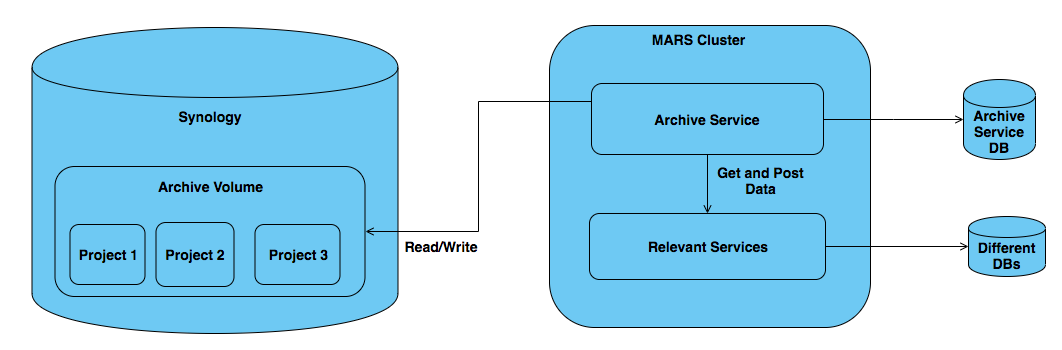
\includegraphics[scale=0.4]{grafiken/synology.png}
                \caption{Archive service's communication structure}
                \label{fig:synology}
            \end{figure}

            Figure \ref{fig:synology} illustrates the communication procedure required to be implemented for the archive and retrieval process. 
            This requirement must be fulfilled to comply with the MARS development standard. As seen, the
            Archive service can read and write directly only to the archive volume in Synology and its own database. The data which is not owned by the archive
            service has to be requested via an API to the relevant service for read/write purposes. The figure generalizes the services it communicates with
            as "Relevant Services" because this diagram only intends to show an abstraction for the communication between them.

        \subsection{Download archived data as a compressed file}
            It is of great importance for a Domain Expert i.e. ecologist to have a graphical interface in hand. In this interface
            it should be possible to navigate to the project of interest and easily download the project as a zip file. There could be cases where the
            MARS system is out of order and the data is required which could then be accessible by anyone with basic knowledge of the system.
        
        \subsection{Design for Failure}   
        Firstly, the Archive service has to communicate with many services in the system, leading the rate of failure being higher
        in comparison to a system which does not depend on other services. A breakdown 
        of one service would cause the whole process of archive/retrieve to stop unexpectedly.  Secondly, it is also possible that a running Archive service be terminated
        due to some unexpected reason. Therefore, fault tolerance mechanism has to be included in the Archive system so that it has a chance of 
        recovery. 

\newpage
\section{Non functional Requirements}
\label{section:technicalReq}
The requirements specified in this section present us the technical/non-functional aspects of the Archive service. A tabular description 
(Table \ref{table: Technical Requirements}) is presented below.
The detailed description depicts the benchmarks of how the system should be designed to meet the needs for a better sustainable prototype.
The result from this work delivered must comply with the following technical requirements.

    \begin{longtable}{|p{3cm}|p{12cm}|}
            \hline
                \textbf{Requirement}  & \textbf{Description}\\
            \hline
                 Build and deployment & 
                 The service should be deployable in the MARS kubernetus \cite{kubernetes} cluster using the Gitlab pipeline as seen in Figure \ref{fig:CIbuild}
                 which is valid at the time of writing this Thesis. In addition,
                 the build stages for the pipeline also has to be written. \\
            \hline
                Docker containerizing.
                & Choose a suitable Docker container \cite[p.~7 - 8]{Torre2017} for the service. This depends on the type of programming language which 
                the service is being
                written in (e.g. dotnet core, python, java, go).\\
            \hline
                 Scalability & Provide further extensibility option using object orientation so that the service can be scalable.\\
            \hline
                 Robustness & The system should be tested against multiple cases to ensure correct functionality of the service using unit tests and
                 integration tests.\\    
            \hline
                 Performance & The duration of the archive and retrieve process should be measurable. So that a close watch on the performance of the system is 
                 possible. \\    
            \hline
                 Usability & The system should be integrated in the MARS UI so that it is easily usable by all end users.\\    
            \hline
                 Connection to Synology & The Archive service should be able to make a connection to the Synology drive and store desired data successfully.\\ 
            \hline
                 Make a Swagger API interface & The Archive service should have a Swagger \cite{swagger} interface available so that other 
                 developers can use the service with ease.\\         
            \hline
                Follow Microservice patterns & The service should follow data sovereignty pattern for Microservices mentioned in 
                (Subsection \ref{subsection:dataSovereignty}).\\ 
            \hline
                Responsiveness & The API should give some kind of feedback to the user never the less if request cannot be made an 
                error message should be returned instead of no result. \\      
            \hline
        \caption{Technical requirements for the Archive service}
        \label{table: Technical Requirements}     
    \end{longtable} 
  
    \begin{figure}[H]
        \centering 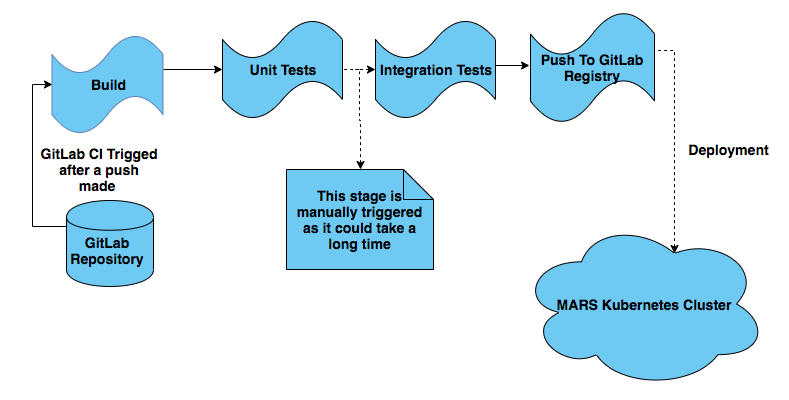
\includegraphics[scale=0.5]{grafiken/CIbuild.png}
        \caption{MARS Continuous Integration Pipeline build}
        \label{fig:CIbuild}
    \end{figure}

    Figure \ref{fig:CIbuild} presents the Continuous Integration system which is being followed at the time of writing this thesis by the MARS developer community.
    The CI\footnote{CI: Continuous Integration} pipeline would be triggered as soon as a new commit is being pushed to the remote 
    GitLab\footnote{https://about.gitlab.com} repository. This would then build the docker image of the service with the new changes. The next step would be to
    run the unit tests written for the service, which is a mandatory step. Lastly, if the pipeline passes, the docker image will be pushed
    to the GitLab registry\footnote{https://about.gitlab.com/2016/05/23/gitlab-container-registry/}. If this is successful then the image can be used in one of 
    the MARS kubernetes cluster i.e. MARS beta, MARS production environments. In addition,
    it can be seen that the integration tests are configured to be an optional test because the integration tests could consume considerably more time and may hinder
    important updates. For this reason, the integration tests are ran manually in the pipeline.
						% chapter 2: Analysis
%---------------------------------------------------------------------------------------------------
% Design
%---------------------------------------------------------------------------------------------------
\newpage
\chapter{Planning And Software Design}
The chapter discusses the decisions, design patterns, architectures, libraries utilized for this thesis, following the requirements mentioned in 
Chapter \ref{chap:ReqAnalysis}.

\section{API Design}
    The Archive service must expose its web APIs to its client so that an interaction between the application can occur.
    The Representational State Transfer (REST) \cite[Chapter.~5]{REST} architectural approach is chosen for this thesis
    to design its API. This approach is a 
    common approach to build a distributed system as it is independent of any system. Therefore using this architecture the system can later 
    evolve for any kind of system which could be used in the future providing a broader layer of flexibility to the Archive service. 
    Also, the standardized aspects of RESTful service enables a software to create a reusable elements \cite{RESTThesis}. A combination of HTTP with REST to carry out
    CURD operations is more preferred since HTTP is widely supported by most clients and programming languages (e.g. web browsers).
    The CURD over HTTP consists of few uniform noun based interaction that can be executed by the client \cite[p.~13]{RESTThesis}. The
    HTTP CURD operations which are going to be implemented are described in Table \ref{table:curdHttp}.

    \begin{table}[h!]
        \centering
        \begin{tabular}{|p{2cm}|p{4cm}|p{7cm}|}
            \hline
                \textbf{HTTP Verb}  & \textbf{Description} & \textbf{Application}\\
            \hline
                POST & 
                Creates a new resources and dependent resources.
                & The POST request will be used to archive and retrieve the projects because new resources are being created for these requests.\\
            \hline
                GET & Reads the resource. & The GET request will be used to check the status of the archive and retrieve process. \\
            \hline
                DELETE & Deletes the resource. & The DELETE request will be used to delete a running archive or retrieve process. \\                
            \hline
        \end{tabular}
        \caption{CURD interaction over HTTP in Archive service}
        \label{table:curdHttp}     
    \end{table}   
    
    Table \ref{table:archiveEndpoints} mentions the API endpoint for archive, retrieve and job status with brief description.
    \begin{table}[H]
        \centering
        \begin{tabular}{|p{6cm}|}
            \hline
                \textbf{API Endpoint}\\
            \hline
                archive/archiveProject/{{projectId}} \\
            \hline
                retrieve/retrieveProject/{{projectId}} \\
            \hline
                job/status/{{projectId}} \\
            \hline
                job/status/{{jobId}} \\
            \hline
        \end{tabular}
        \caption{API Endpoints description for Archive service}
        \label{table:archiveEndpoints}     
    \end{table}   


    

\section{Archive Process Design}
\subsection{Preconditions Required for an Archive}
Certain preconditions have to be met before an archive process could start to ensure the correctness of the data which are mentioned below:
\begin{enumerate}
    \label{lst:preconditionsArchive}
    \item \textbf{Mark resources:} The MARS framework is a multi user application meaning a project can be accessed by many users at the same time. 
    As multiple users can modify the data simultaneously, it could be possible that someone changes a resource during an archive and the 
    Archive service has no way to detect this modification. This would lead to inconsistent data being archived.
    Therefore, to avoid this situation the resources must be marked before the start of an archive. The marking would ensure that no other process except the Archive
    service would have access to modify the marked contents during the archive process. The marking process would be handled using the Marking service.
    \item \textbf{Get Metadata for the project:} The metadata contains all necessary information about
    the different resources. The scenarios, files and the result configuration depend on these metadata
    to retrieve their respective data. If the metadata cannot be obtained the archive process cannot continue.
    \item \textbf{Get Simulation runs:} The simulation run contains the simulation id which is required to archive the correct simulation. This dependency
    with simulation run makes it necessary that they are obtained before archiving the simulation results.
\end{enumerate}

\subsection{Decision for Not Archiving the Project}
The resources depicted in table (Table \ref{table: archivedMars}) must be archived following the MARS resource hierarchy (Figure \ref{fig:marsDependency}).
Following the hierarchy, it is arguable why the project is not being archived, despite it being present. The project lies on the top of the hierarchy 
meaning no other resources are usable without its existence. Section \ref{ssec:retrieveAnalysis} mentions the requirement that the Archive service must 
restore all the archived resources back into the system. Therefore, during a restore, if a specific archived project
is not available, then other resources cannot be brought back into the system as all of them are dependent to the project. To make the restore process possible,
the project data is not archived which now acts as a point of reference to bring back the children resources. 
If the project was to be archived then additionally a mechanism is needed that ensures the users referenced in the archive also exist in the Mars system (active system).
It could be possible that during a retrieve the users in an
archived project may not exist anymore as they were removed causing the process to fail. Therefore, this decision also reduces the complexity of the 
archive and restore as this mechanism can be avoided.


\subsection{Data Format}
A suitable file format for archiving must be chosen because it determines how the data access will be realized and whether it meets
the criteria mentioned in Section \ref{section:functionalReq}. The different types of data archived are the metadatas for files, scenarios, 
result configurations, simulation plans, simulation run including the input files, models, and the simulation results. 
The data format that is being discussed in this section mainly focuses on the metadata and they are received originally as a JSON document.
The metadata is very important because they give the system vital information that will be used during retrieve process. 

\subsubsection{HDF5}
HDF5 is a file format for storing and managing data which has support for various data types designed for
efficient I/O, compression, portability and, supports big data \cite{HDF5}. It has been successfully applied to different scientific projects which
involve simulation (Efficient
for simulation data \cite[p.~11]{Savic2007}). This file can also be defined as an abstract data container which includes building blocks for data organization. 
This file system can hold a variety of heterogeneous objects like images, graphs, documents, tables etc. It also has support for a n-dimensional table  \cite[p.~2]{HDF5}. 
The HDF5 format has two primary objects which define the data storage structure:
\begin{enumerate}
    \item \textbf{Groups:}  They are responsible to organize the data objects in the HDF5 file format. A Group can be compared to a directory 
    in Windows or Unix system \cite{HDF5}. Figure \ref{fig:HDF5} shows an example of a Group (e.g. project1) in a HDF5 file. Using the API of the HDF5 libraries a Dataset 
    (e.g. scenario Metadata) can be accessed via the path name (e.g. /Root/project1/scenario Metadata).
    \item \textbf{Datasets:} A Dataset can be defined as a multidimensional array of data. This object contains the raw/actual data (e.g. simulation results).
    These data are stored in a n-dimensional array format, where 
    one can specify the different data types for the raw data i.e. integer, float, character, variable length strings \cite{HDF5}. Figure \ref{fig:dataset} shows
    an example of a Dataset in a HDF5 file which is stored in an array.
\end{enumerate}

Figure \ref{fig:HDF5} also shows how the Groups and Datasets can be used to archive the MARS projects. Every new project to be archived will be added as a new Group
as depicted in the figure and the datasets are the resources i.e. scenario, file, simulation results. 

\begin{figure}[H]
    \centering 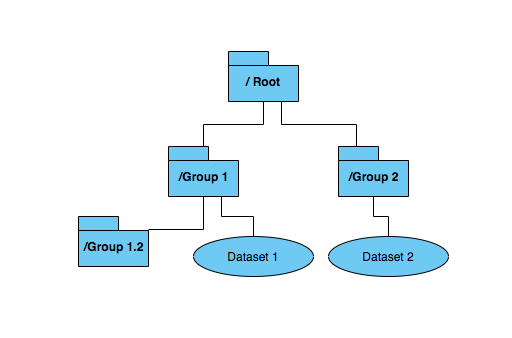
\includegraphics[scale=0.6]{grafiken/groupsHDF5.png}
    \caption{HDF5 Groups and Datasets \cite{HDF5}}
    \label{fig:HDF5}
\end{figure}

\begin{figure}[H]
    \centering 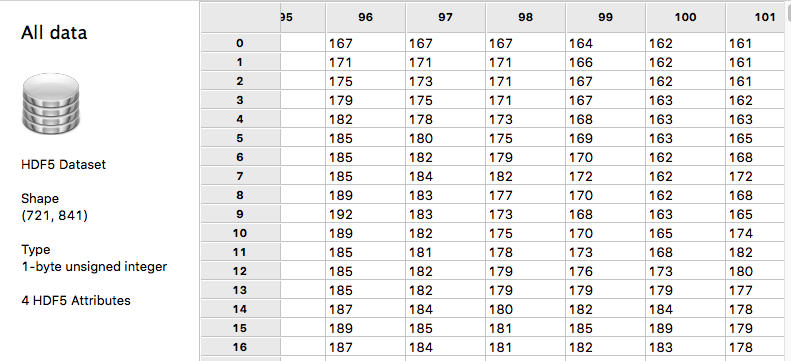
\includegraphics[scale=0.45]{grafiken/dataset.png}
    \caption{Example of a HDF5 dataset}
    \label{fig:dataset}
\end{figure}

\subsubsection{JSON} 
JSON(JavaScript Object Notation) is a data format which is very easy for humans and machines to read and write. This format is
completely language independent which follows the conventions used in different programming languages i.e. C\#, Java, Python and more. The REST API implemented in the
MARS framework supports this format with ease making this a very suitable candidate. This format is widely 
accepted and even MongoDB supports it without any problem. Also, MongoDB seems to be a good candidate but the requirement (Section \ref{sec:anaCompress}) states that the archived
data should be easily accessible to a non expert and using MongoDB requires some amount of technical expertise.


\subsubsection{Conclusion}
   %The HDF5 is a very powerful file format providing more efficient data storage and lookup by separating its raw data with its metadata. 
    To store the data in HDF5 all the attributes of the metadata in JSON must be parsed in a n-dimensional array structure which can be understood by the HDF5. 
    It is important to understand that MARS supports different kind of models which makes it impossible to predict the structure of a resource. To elaborate, the
    Wolves and Sheep \cite{HAWHamburgMARS} model has a different metadata structure than the KNP \cite{HAWHamburgMARS} model as the Agents and Layers involved are 
    different. Due to this reason, the resources
    must be parsed every time into a n-dimensional array by writing each field. Also, at the time of restore this has to be converted back 
    to a JSON as the MARS system does not understand the HDF5 structure. In addition, to avoid parsing the data, 
    a one dimensional array of size 1 was created (type variable string) and all the unparsed JSON data
    was stored in this array. The main intention of this experiment was to see how the HDF5 files would react as it is easy to get the string from a 1d array 
    (e.g. exprimentArray[0]). This also did not bring any positive result, instead it created so much overhead to the file as a JSON file with the size of 2 KB
    had a file size of around 0.5MB for the HDF5 variant. This made the HDF5 file system very inconvenient to use.
    Despite the HDF5 file providing different benefits i.e. fast I/O, portability, support for big data and,
    compression on a dataset it does not seem suitable in the MARS system due to the amount of complexity that needs to be dealt with for the archive and restore process.
    

    Considering the above mentioned factors the file format for the metadata is planned to be JSON instead of the HDF5 file. Different advantages such as easy 
    handling, no extra parsing
    required for the MARS system and, easy conversion to different types of file format i.e. CSV used often in the MARS for analysis, makes it more suitable for this purpose. 
    To aid the performance, the meta files for each kind of resources
    are going to be stored separately (e.g. scenario.json, resultConfiguration.json). Splitting the JSON files like this would aid in faster serialization and 
    deserialization as only the required resource can be loaded into the memory. As the input files and the simulation results do not need to be read they are just chosen to be zipped.

\begin{figure}[H]
    \centering 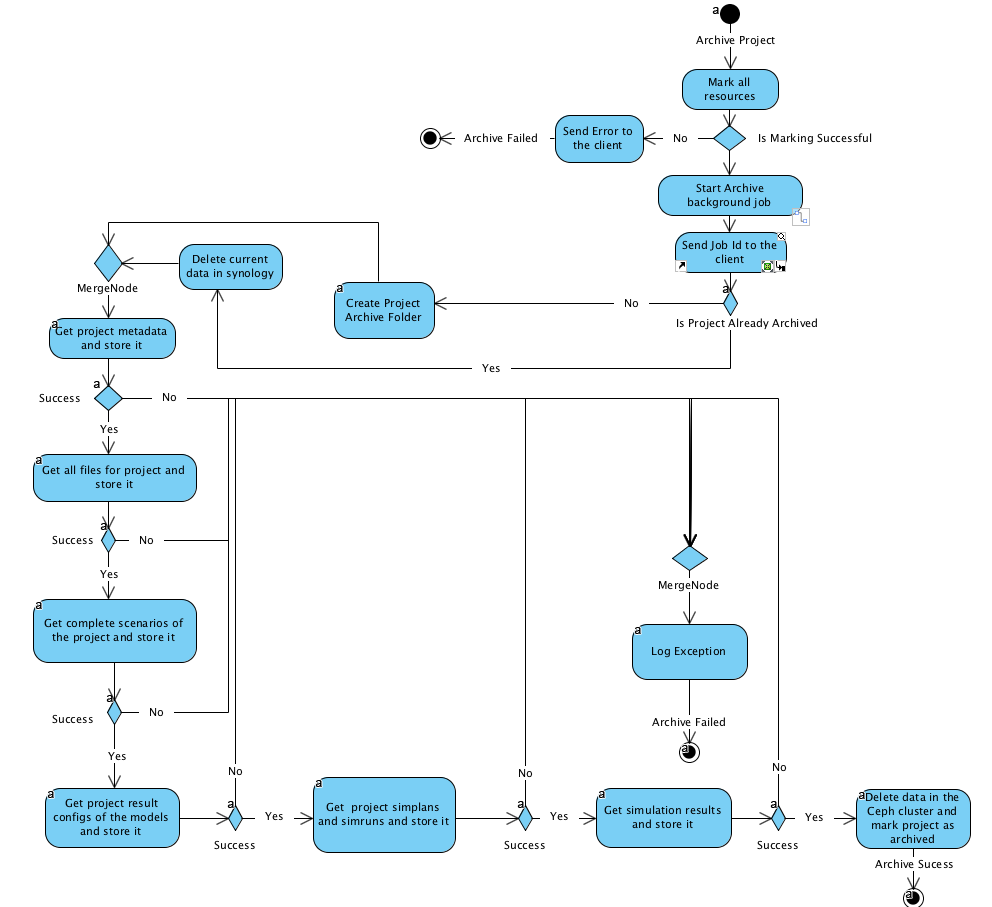
\includegraphics[scale=0.45]{grafiken/archiveActivity.png}
    \caption{Activity Diagram of MARS project Archive process}
    \label{fig:archiveActivity}
\end{figure}

Figure \ref{fig:archiveActivity} illustrates an activity diagram of archiving an entire project in the MARS system. As mentioned in Section \ref{lst:preconditionsArchive},
marking the resources for the project is the first requirement needed to start the process. If the project resources are marked successfully
then the archive would be initialized as a background job and the job id would be sent to the client. In case the marking would fail, the error message will be 
sent to the client and the archive process will halt. The archiving process is visioned to be a background job due to the fact that a single process could take
a long period of time and would block the server for additional requests. Following the successful job creation, the process checks if an archive already
exists. After
the archive folder creation, the metadata, files, scenarios, result configurations, simulation plans, simulation runs, and the simulation results are retrieved respectively.
After a successful archive process the  resources are deleted from the Ceph cluster. Lastly, in case of some failures during archiving the exception will be logged 
which can be later analyzed for maintenance.

\begin{figure}[H]
    \centering 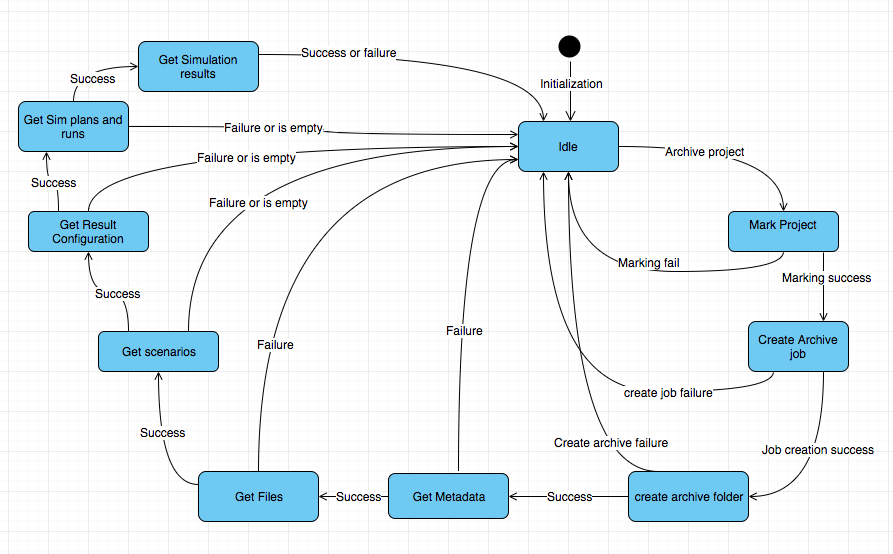
\includegraphics[scale=0.45]{grafiken/stateArchive.png}
    \caption{State Diagram of MARS project Archive process considering empty states}
    \label{fig:stateArchive}
\end{figure}

Figure \ref{fig:stateArchive} illustrates the transitions that can occur during the archive process. The idle state is when no archive process
is being executed. Additionally, the state digram also considers
how the state would change if one of the resources is empty. In the case of an empty resource (e.g. no scenarios available for the project) the archive
process stops gracefully by logging the error and transitions to the idle state. 

\begin{figure}[H]
    \centering 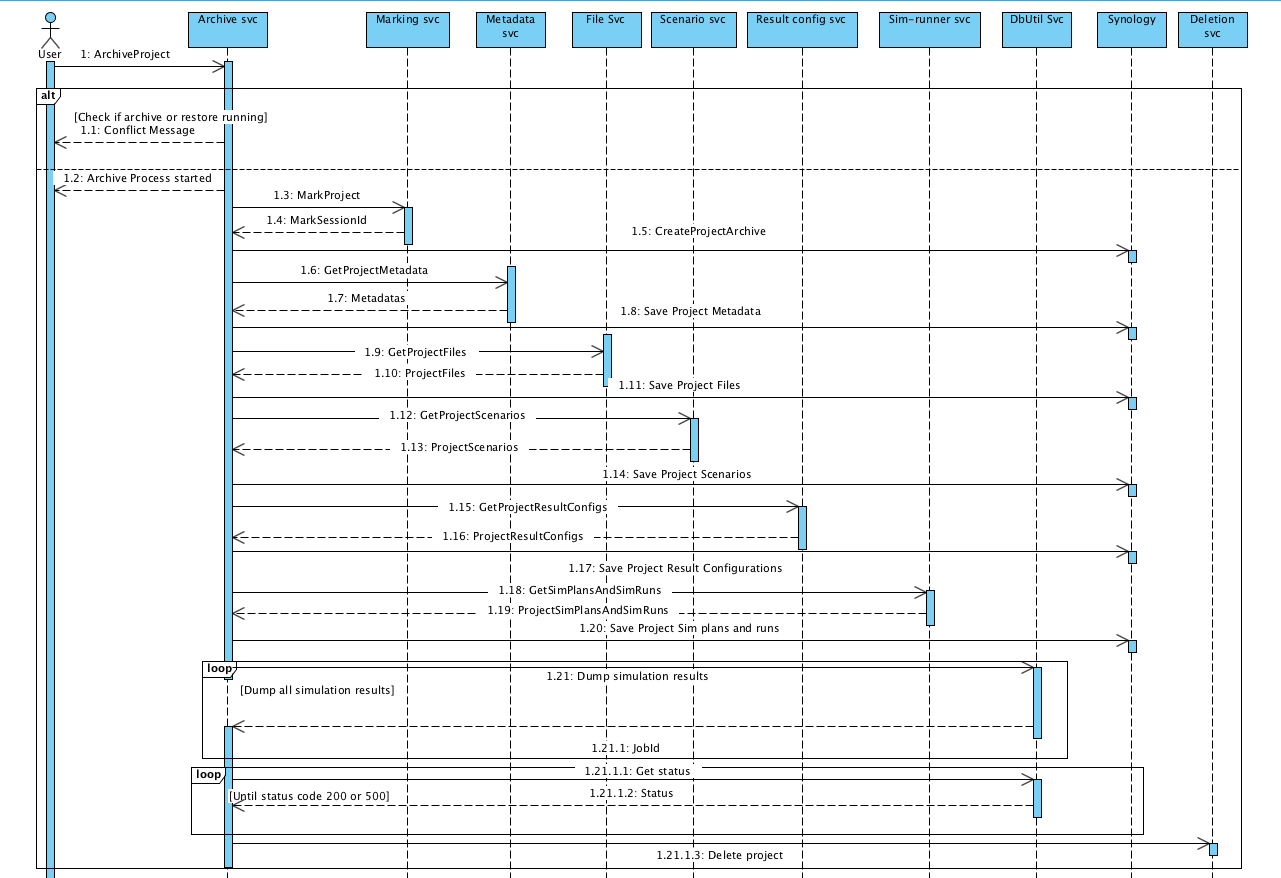
\includegraphics[scale=0.5, angle=90, origin=c]{grafiken/sequenceArchive.png}
    \caption{Sequence Diagram for the Archive process}
    \label{fig:sequenceArchive}
\end{figure}

Figure \ref{fig:sequenceArchive} illustrates the Sequence diagram for a complete archive process. The first step after an archive request would be to check
whether an archive or retrieve process for the current project is under progress. In case the process is in progress, the archive request would be denied to the
user with a conflict message. If no process with the project is running then an archive job (a separate thread) would be created and a message to the client with start of archive process would be
sent. Following the job creation, the project will be marked so that during archive no changes to the project resources could be made. If this step fails the archive 
process would stop by logging the error. After the marking step completes, the archive process receives a mark session id and the dependent resources which would allow the process to make
changes to the resources. Using the dependent resources the process retrieves metadata, files, scenarios, result configurations, simulation plans and, simulation runs 
respectively and persists them in Synology. Lastly, the simulation result dump action will be called which will archive the result data. The process waits until
all the result data is archived successfully. After a successful archive, a request to delete the project data would be made so that the system memory can be freed.

A major issue to be discussed is when the archive process fails which requires a rollback by unmarking the project. As mentioned earlier the project is
marked as "TO\_BE\_ARCHIVED" so that no other processes can modify the contents during the archive process. This is a great strategy if everything goes as planned but 
often this is not the case, and it is mandatory that an unmarking of the project is done otherwise the project would be unusable. 

It also happens that since the
marking service is dependent upon many services, it has a high possibility of failure as well. This brings upon the problem how would the archive service behave if the
unmarking of the project fails. It seems very natural to just repeat the process until the unmarking request would succeed, since it is absolutely necessary to unmark
a project. If this happens only with a single process, it does not make a huge difference. However when thinking of the bigger picture if this 
occurs with 100 different processes at the same time, it would use valuable processing resources as it may be stuck in a deadlock condition until a outside interruption
is made. To avoid this, a fixed number of retries to unmark the project with certain time interval for the request 
will be made. 

Although, this solves the issue of using up resources but the problem that the project is unusable is still there. Except a manual unmarking, no other solution 
can be seen, so 
it is decided that the archive process would also persist the marking session id which can be used to call the unmarking endpoint. With the use of this id a manual 
trigger is possible as soon as the error is fixed. The marking session id can be easily retrieved also from the GUI as it will be included in the status request of
the archive job.
 
\section{Architecture Design Patterns}

\subsection{Decision for Dotnet framework}
\label{ssec:dotnet}

MVC\footnote{MVC: Model View Controller} is one of the many architectural patterns, which provide a common reusable solution in a software system.
This is presumably by far the most used designed pattern adapted by many frameworks like
Microsoft .NET core MVC, 
Java Spring framework MVC etc. 

\begin{figure}[H]
    \centering 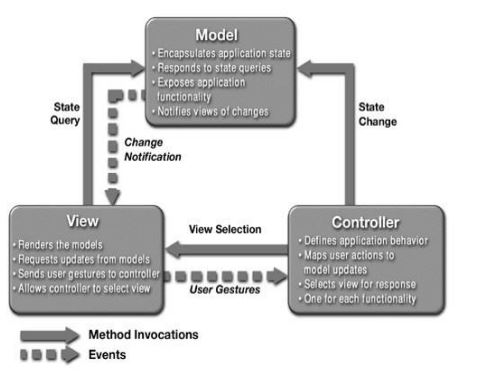
\includegraphics{grafiken/mvc_hotop.jpg}
    \caption{MVC Overview \cite{Hotop2015}}
    \label{fig:mvcOverview}
\end{figure}

\par
   The main idea behind is to make a clear separation between domain object and the presentation layer. The two elements should be completely self-
   contained and should be able to work without the presence of the other. This 
   architecture acknowledges three primary aspects. Figure \ref{fig:mvcOverview} 
   gives us an overview of MVC pattern.
   \begin{enumerate}
       \item 
        \textbf{The Model}: This is the layer which represents the data layer. It 
        contains all the relevant data for the business logic.

       \item 
        \textbf{The View}: This is the user interface where the graphical units area
        placed like buttons, text etc.

       \item 
        \textbf{The Controller} : This layer takes the inputs and changes the two other
        layer accordingly.
   \end{enumerate} 

    


							% chapter 3: Design
%---------------------------------------------------------------------------------------------------
% Realisation
%---------------------------------------------------------------------------------------------------
\newpage
\chapter{Realisation}
And here the real realisation is outlined, this is your part... a lot of figures?
	% Chapter 4: Realisation

%---------------------------------------------------------------------------------------------------
% Thrd art of the thesis
%---------------------------------------------------------------------------------------------------
%	%---------------------------------------------------------------------------------------------------
%end
%---------------------------------------------------------------------------------------------------
\newpage
%\part{end}
\chapter{Conclusion}
The last important words...
																								
%---------------------------------------------------------------------------------------------------	
%references
%---------------------------------------------------------------------------------------------------		
	
\renewcommand{\bibname}{References}
\bibliographystyle{abbrv}    
\bibliography{literatur/literatur}   														% reference list
% references added but need not be referenced inside the text
% references used inside the text with  \nocite or \cite must be added to the .bib File!

\nocite{HAWHamburgMARS}
\nocite{Torre2017}
\nocite{Savic2007}
\nocite{Heber2014}
\nocite{Holzmann2016}
\nocite{Heber2014a}
\nocite{Newman2015}
\nocite{Synology}
\nocite{DistributedSystems}
\nocite{DDD}
\nocite{SOA}
\nocite{MicroserviceNewMan}
\nocite{FowlerMartin}
\nocite{GIS}
\nocite{Timeseries}
\nocite{MongoDB}
\nocite{agentModeling}
\nocite{Ceph}
\nocite{softwareDesign}
\nocite{Haerder1983}
\nocite{TrafficModel}
\nocite{Grundmann2018}
\nocite{CAP}
\nocite{grpc}
\nocite{HTTP}
\nocite{Polyglot}
\nocite{kubernetes}
\nocite{REST}
\nocite{RESTThesis}
\nocite{swagger}
\nocite{Hotop2015}
\nocite{WARC}
\nocite{MARSCLoud}
\nocite{Hangfire}
\nocite{Hangfire}
\nocite{atomic}																				%add the non refeenced papers or literature which are as well important for the thesis!

%---------------------------------------------------------------------------------------------------	
% appendix
%---------------------------------------------------------------------------------------------------	
	\appendix
% \input{anhang/hilfsmittel/hilfsmittel}															% appendix A: helps for the implementation
																																			% 					of this thesis
%	\input{anhang/quellcode/quellcode}																	% Appendix B: SourceCode

%---------------------------------------------------------------------------------------------------	
% Glossar
%---------------------------------------------------------------------------------------------------	
	\printnomenclature

%---------------------------------------------------------------------------------------------------	
% index
%---------------------------------------------------------------------------------------------------	
	\printindex
	
%---------------------------------------------------------------------------------------------------	
% Declaration
%---------------------------------------------------------------------------------------------------		
	\asurency	

%--------------------------------------------------------------------------------------------------- 
% End of the thesis
%--------------------------------------------------------------------------------------------------- 
\end{document}
